\begin{figure} [h]
    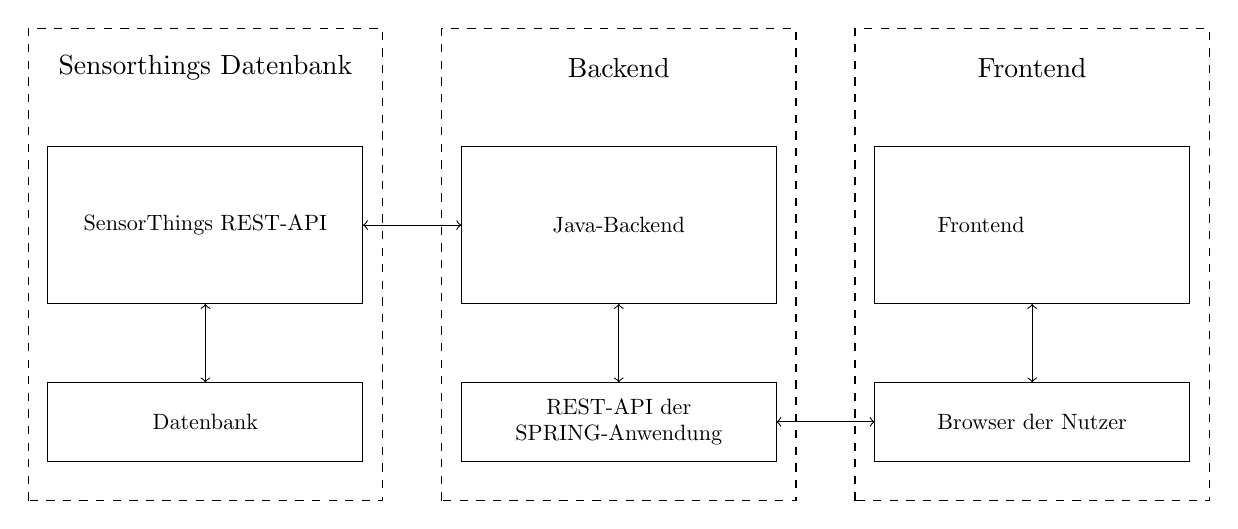
\begin{tikzpicture}[node distance=2cm]

        %Model
        \begin{scope}[shift={(0,0)},local bounding box=SensorThings]
            \draw (0,0) [dashed] rectangle (4.5,6);
            \node[scale=1] at (2.25,5.5) {Sensorthings Datenbank};
            \begin{scope}[local bounding box=API]
                \draw (0.25,2.5) rectangle (4.25,4.5);
                \node[scale=0.8] at (2.25,3.5) {SensorThings REST-API};
            \end{scope}
            \begin{scope}[local bounding box=Datenbank]
                \draw (0.25,0.5) rectangle (4.25,1.5);
                \node[scale=0.8] at (2.25,1) {Datenbank};
            \end{scope}
        \end{scope}
        
        %Controller
        \begin{scope}[shift={(5.25,0)},local bounding box=Backend]
            \draw (0,0) [dashed] rectangle (4.5,6);
            \node[scale=1] at (2.25,5.5) {\softwarename Backend};
            \begin{scope}[local bounding box=VisAQBackend]
                \draw (0.25,2.5) rectangle (4.25,4.5);
                \node[scale=0.8] at (2.25,3.5) {\softwarename Java-Backend};
            \end{scope}
            \begin{scope}[local bounding box=BackendAPI]
                \draw (0.25,0.5) rectangle (4.25,1.5);
                \node[scale=0.8, align=center] at (2.25,1) {REST-API der\\SPRING-Anwendung};
            \end{scope}
        \end{scope}

        %View
        \begin{scope}[shift={(10.5,0)},local bounding box=Frontend]
            \draw (0,0) [dashed] rectangle (4.5,6);
            \node[scale=1] at (2.25,5.5) {\softwarename Frontend};

            \begin{scope}[local bounding box=VisAQFrontend]
                \draw (0.25,2.5) rectangle (4.25,4.5);
                \node[scale=0.8,text width=3cm] at (2.25,3.5) {\softwarename Frontend};
            \end{scope}
            \begin{scope}[local bounding box=Browser]
                \draw (0.25,0.5) rectangle (4.25,1.5);
                \node[scale=0.8] at (2.25,1) {Browser der Nutzer};
            \end{scope}
        \end{scope}

        \draw[<->] (API.south) -- (Datenbank.north);
        \draw[<->] (API.east) -- (VisAQBackend.west);
        \draw[<->] (BackendAPI.north) -- (VisAQBackend.south);
        \draw[<->] (BackendAPI.east) -- (Browser.west);
        \draw[<->] (VisAQFrontend.south) -- (Browser.north);

    \end{tikzpicture}
    \caption{Diagramm des Gesamt-Systems}
\end{figure}